
\section{Introduction to Organization}
\subsection{Testing and Consutancy Cell}
\begin{figure}[ht]
\centering
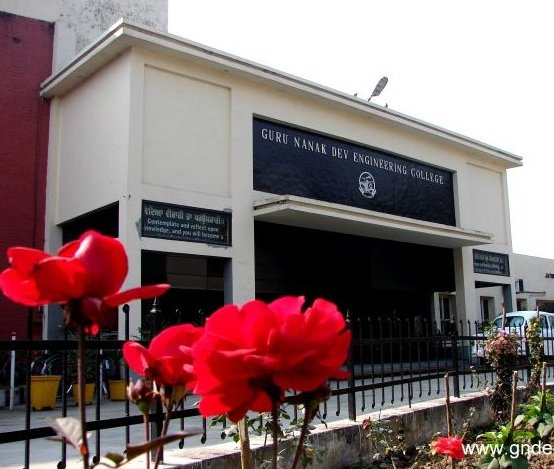
\includegraphics[scale=0.5]{input/images/gndec.jpg}
\caption{Guru Nanak Dev Engineering College}
\end{figure}
\hspace{-1.7em} 
\noindent I attended starting 2 months of my training at TCC i.e. Testing and Consultancy Cell, GNDEC Ludhiana
under the guidance of Dr. H.S. Rai Dean Testing and Consultancy Cell from 6 th June 2017 to 8 th August
2017.\\

\noindent Testing and Consultancy Cell was established in the year 1979 with a basic aim to produce quality
service for technical problems at reasonable and affordable rates as a service to society in general and
Engineering fraternity.\\

\noindent Consultancy Services are being rendered by various Departments of the College to the
industry, Sate Government Departments and Entrepreneurs and are extended in the form of
expert advice in design, testing of materials \& equipment, technical surveys, technical audit,
calibration of instruments, preparation of technical feasibility reports etc.
This consultancy cell of the college has given a new dimension to the development
programmers of the College. Consultancy projects of over Rs. one crore are completed by the
Consultancy cell during financial year 2009-10. \\


The main goal of this institute is:
\begin{itemize}
\item To build and promote teams of experts in the upcoming specialisations.
\item To promote quality research and undertake research projects keeping in view their
relevance to needs and requirements of technology in local industry.
\item To achieve total financial independence.
\item To start online transfer of knowledge in appropriate technology by means of establishing multipurpose resource centres.
\end{itemize}

Ours is a pioneer institute providing Consultancy Services in the States of Punjab, Haryana,
Himachal, J\&K and Rajasthan. Various Major Clients of the Consultancy Cell are as under:\\
\begin{itemize}
\item Northern Railway, Govt. of India
\item Indian Oil Corporation Ltd.
\item Larson \& Turbo.
\item Multi National Companies like AFCON \& PAULINGS.
\item Punjab Water Supply \& Sewage Board
\end{itemize}
\subsection{Techno Campus}
\begin{figure}[ht]
\centering

\includegraphics[scale=0.5]{input/images/techno.png}
\caption{Techno Campus Logo}
\end{figure}
I attended my next two months of training from 8 th Aug 2017 to 10 Oct 2017 at Techno Campus, Ludhiana.
Techno Campus is a respected learning solutions provider. We are dedicated to creating success stories for
our customers. Our unique integrated learning solution is a proven approach and can be customised to your
individual training needs, be it in the areas of Technical Training, Desktop Applications Training,
Professional Development Training.
\subsection{Numitech Solutions}
\begin{figure}[ht]
\centering

\includegraphics[scale=0.5]{input/images/numi.jpeg}
\caption{Numitech Solutions Logo}
\end{figure}
\noindent The remaining two months of training was attended at Numitech Solutions from 1 st Nov 2017 to 31 st Dec
2017. Numitech Solutions (ISO 9001:2008 Certified) is a prime name in the field of Website Development
and Designing Services / 6 Months and 6 Weeks Industrial Training / Engineering College and School
Projects for all Streams. Established Since 2010, In business hub (Feroze Gandhi Market) center of
Ludhiana, we keep accelerating our company at exponential rate to achieve a good reputation in Market.
We Provide Training and Projects to More than 2000 Students each Year.\\

\noindent Our Key Focus is on providing a Best Quality Service, High end Solutions for Industry and a Great Learning
Experience with total practical approach for students to relate their skills with industrial benchmarks. We
provide Tech Solutions for Lots of Technologies Like Website Design and Development, Software
Development, Embedded, Wireless, Mechanical, Automation, PLC, VLSI, MATLAB, Linux, Java, PHP,
Solar Projects, Android OS, Robotics etc.\\

\noindent We’re a Team of Highly skilled, zealous, enthusiastic, devoted and Experienced people with strong work
ethics who believe in doing what we love and giving full freedom for creativity for each project We believe
Our success lies in Our Clients and Students success. So, we take each client business and each student
Project / Training Very seriously, because fortune of our company is in future of our client.